\begin{frame}
  \frametitle{Logical planning}
  \begin{itemize}
  \item Bipartite query graph -- RA operations/relations unified for all queries
  \item Join ordering enumeration
  \item QNF -- \(\pi \sigma (Q_1 \times Q_2 \times \dots )\) or
    \(\gamma \sigma (Q_1 \times Q_2 \times \dots )\)
  \item Relation shape propagation -- cardinality, columns/types, unique subtuples
  \end{itemize}

\end{frame}

\begin{frame}
  \frametitle{Reversible operators}
  \begin{columns}
    \begin{column}{0.5\textwidth}
      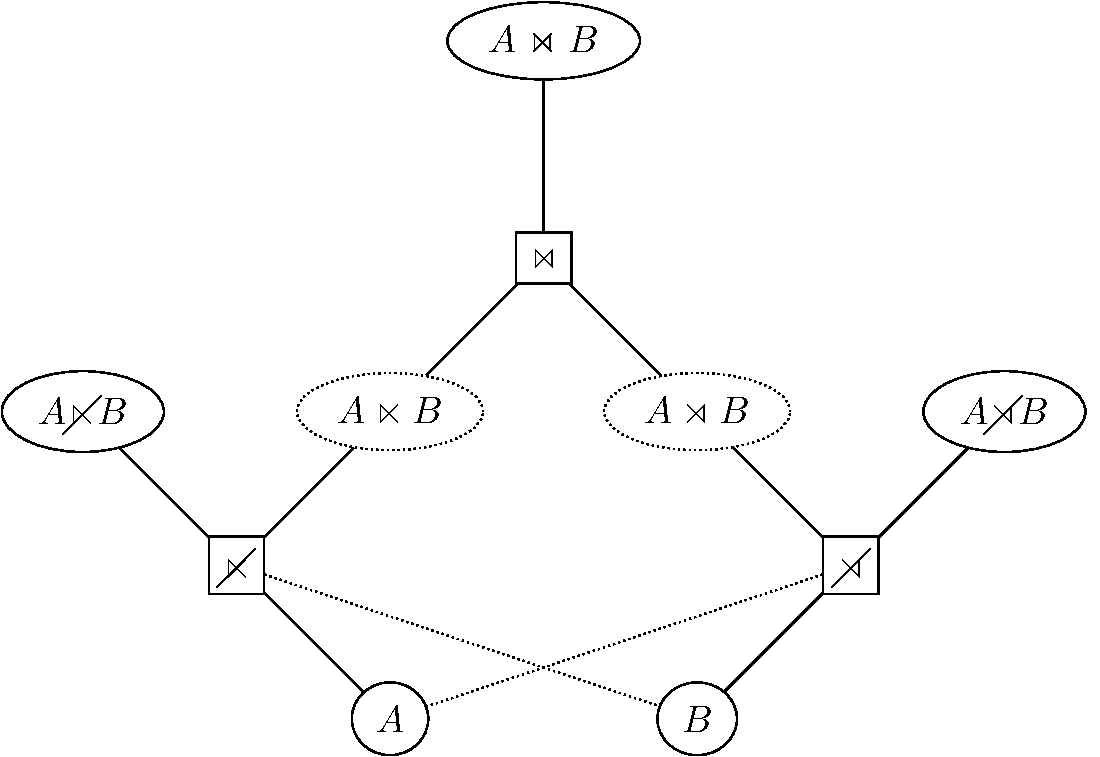
\includegraphics[width=.9\linewidth]{../imgs/joinnet.pdf}
   \end{column}
    \begin{column}{0.5\textwidth}
      \begin{tikzdiagram_w}
        \tikzset{node distance=2cm}
        \tikzset{nnode/.style={ellipse,draw}}
        \tikzset{tnode/.style={rectangle,draw}}

        \node[tnode] (t) {\(\sigma_p\)};
        \node[nnode] (o2) [above left of=t] {\(o_{sec}\)};
        \node[nnode] (o1) [above right of=t] {\(o_{prim}\)};
        \node[nnode] (i) [below of=t] {\(i\)};

        \path (t) edge (i);
        \path (t) edge (o1);
        \path (t) edge (o2);
      \end{tikzdiagram_w}
    \end{column}
  \end{columns}
\end{frame}

\begin{frame}
  \frametitle{Reversible operations}
  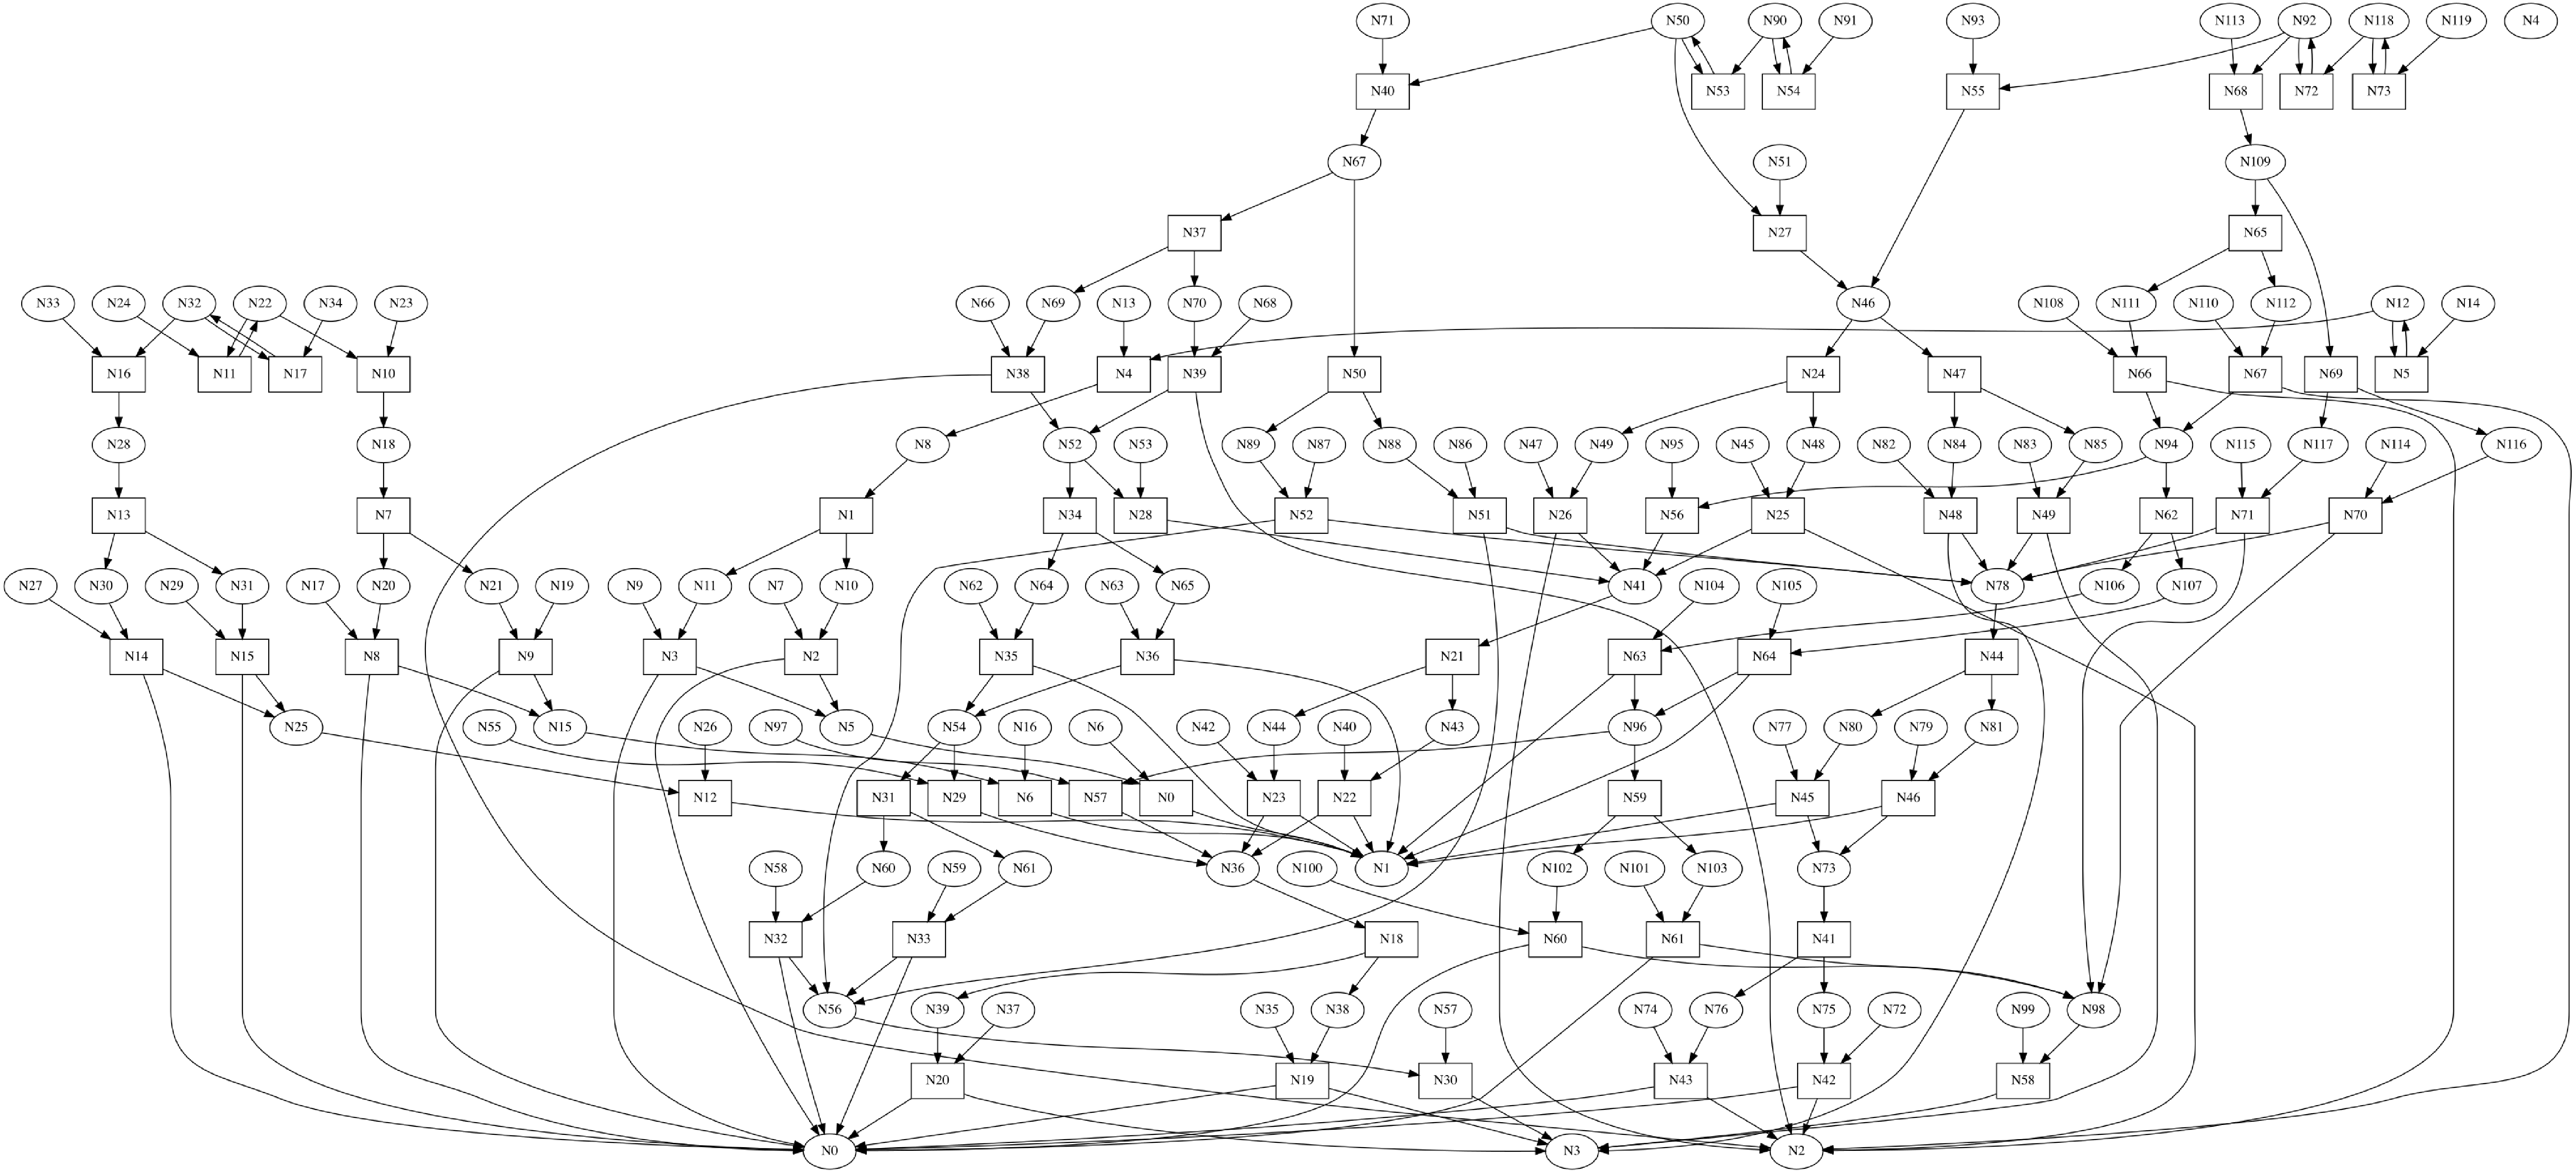
\includegraphics[width=\textwidth]{../imgs/ssb_graph.pdf}
\end{frame}



%%% Local Variables:
%%% mode: latex
%%% TeX-master: "presentation"
%%% End:
